\chapter{Evaluation of Distributed MCTS Algorithms}

\todo{Úvod ke kapitole, co tu bude atd..}

\section{Ms Pac-Man vs Ghosts Framework}

For the purposes of evaluation of algorithms proposed in Chapter \ref{chap_dmcts_design}, we
have chosen the Ms Pac-Man vs Ghosts Framework (\ref{PacmanVsGhosts}) which is easy-to-use
framework allowing implementation of players for well-known old game Pac-Man in Java. Here we
will extract basics of the game rules used in the framework and afterwards we will
describe modifications of the rules we have done and reasons for them.

\subsection{Game rules}

Ms Pac-Man is a game played in a maze in which two sides compete, the Pac-Man and four ghosts.
There are pills everywhere in the maze and Pac-Mans purpuse is to gather all the pills, each
for 10 points. Once all the pills are eaten, the game continues in a next maze. To complicate
the life of Pac-Man, ghosts are moving around the maze pursuing the Pac-Man and trying to
minimize its score. If the Pac-Man is caught, it will lose one life and if has any life
remaining, starts again from its starting position. Pills remain eaten after the life loss.
Ghosts appear in so-called lair at the beginning of each round and after Pac-Man's life loss
from where they start after a several time (different for each ghost). Beside regular pills,
each maze contains four power pills which are awarded with 50 points and when eaten by Pac-Man,
ghosts become edible and twice slower for certain period of time. Pac-Man can eat ghosts during 
this period for
reward of 200 points for first eaten ghost and 400, 800 and 1600 points for other ghosts.
Eaten ghost starts in lair again.

Exact rules of the Ms Pac-Man vs Ghosts game can be found on the project webpage. The game was
additionally modified for purposes of testing of our algorithms. Biggest change of rules is
removing power pills from the mazes together with entire edible ghosts mechanism. Reason for
this decision is lowering the variability of results. When Pac-Man is pursuing edible ghosts,
there is big difference in score when it eats different number of ghosts. For the same reason
three more modification have been done. Pac-Man has only one life, game ends after the first
maze is cleared and random ghosts' reversal is suppressed what is a rule
which adds stochasticity to the game. If the rule is on, there is a 0.15\% probability each tick of
a game that all
ghosts accidentally change their direction. \todo{max. délka hry}
An example of a situation from the game without
power pills is depicted by Figure \ref{fig_pacman_framework}.

\begin{figure}
\begin{center}
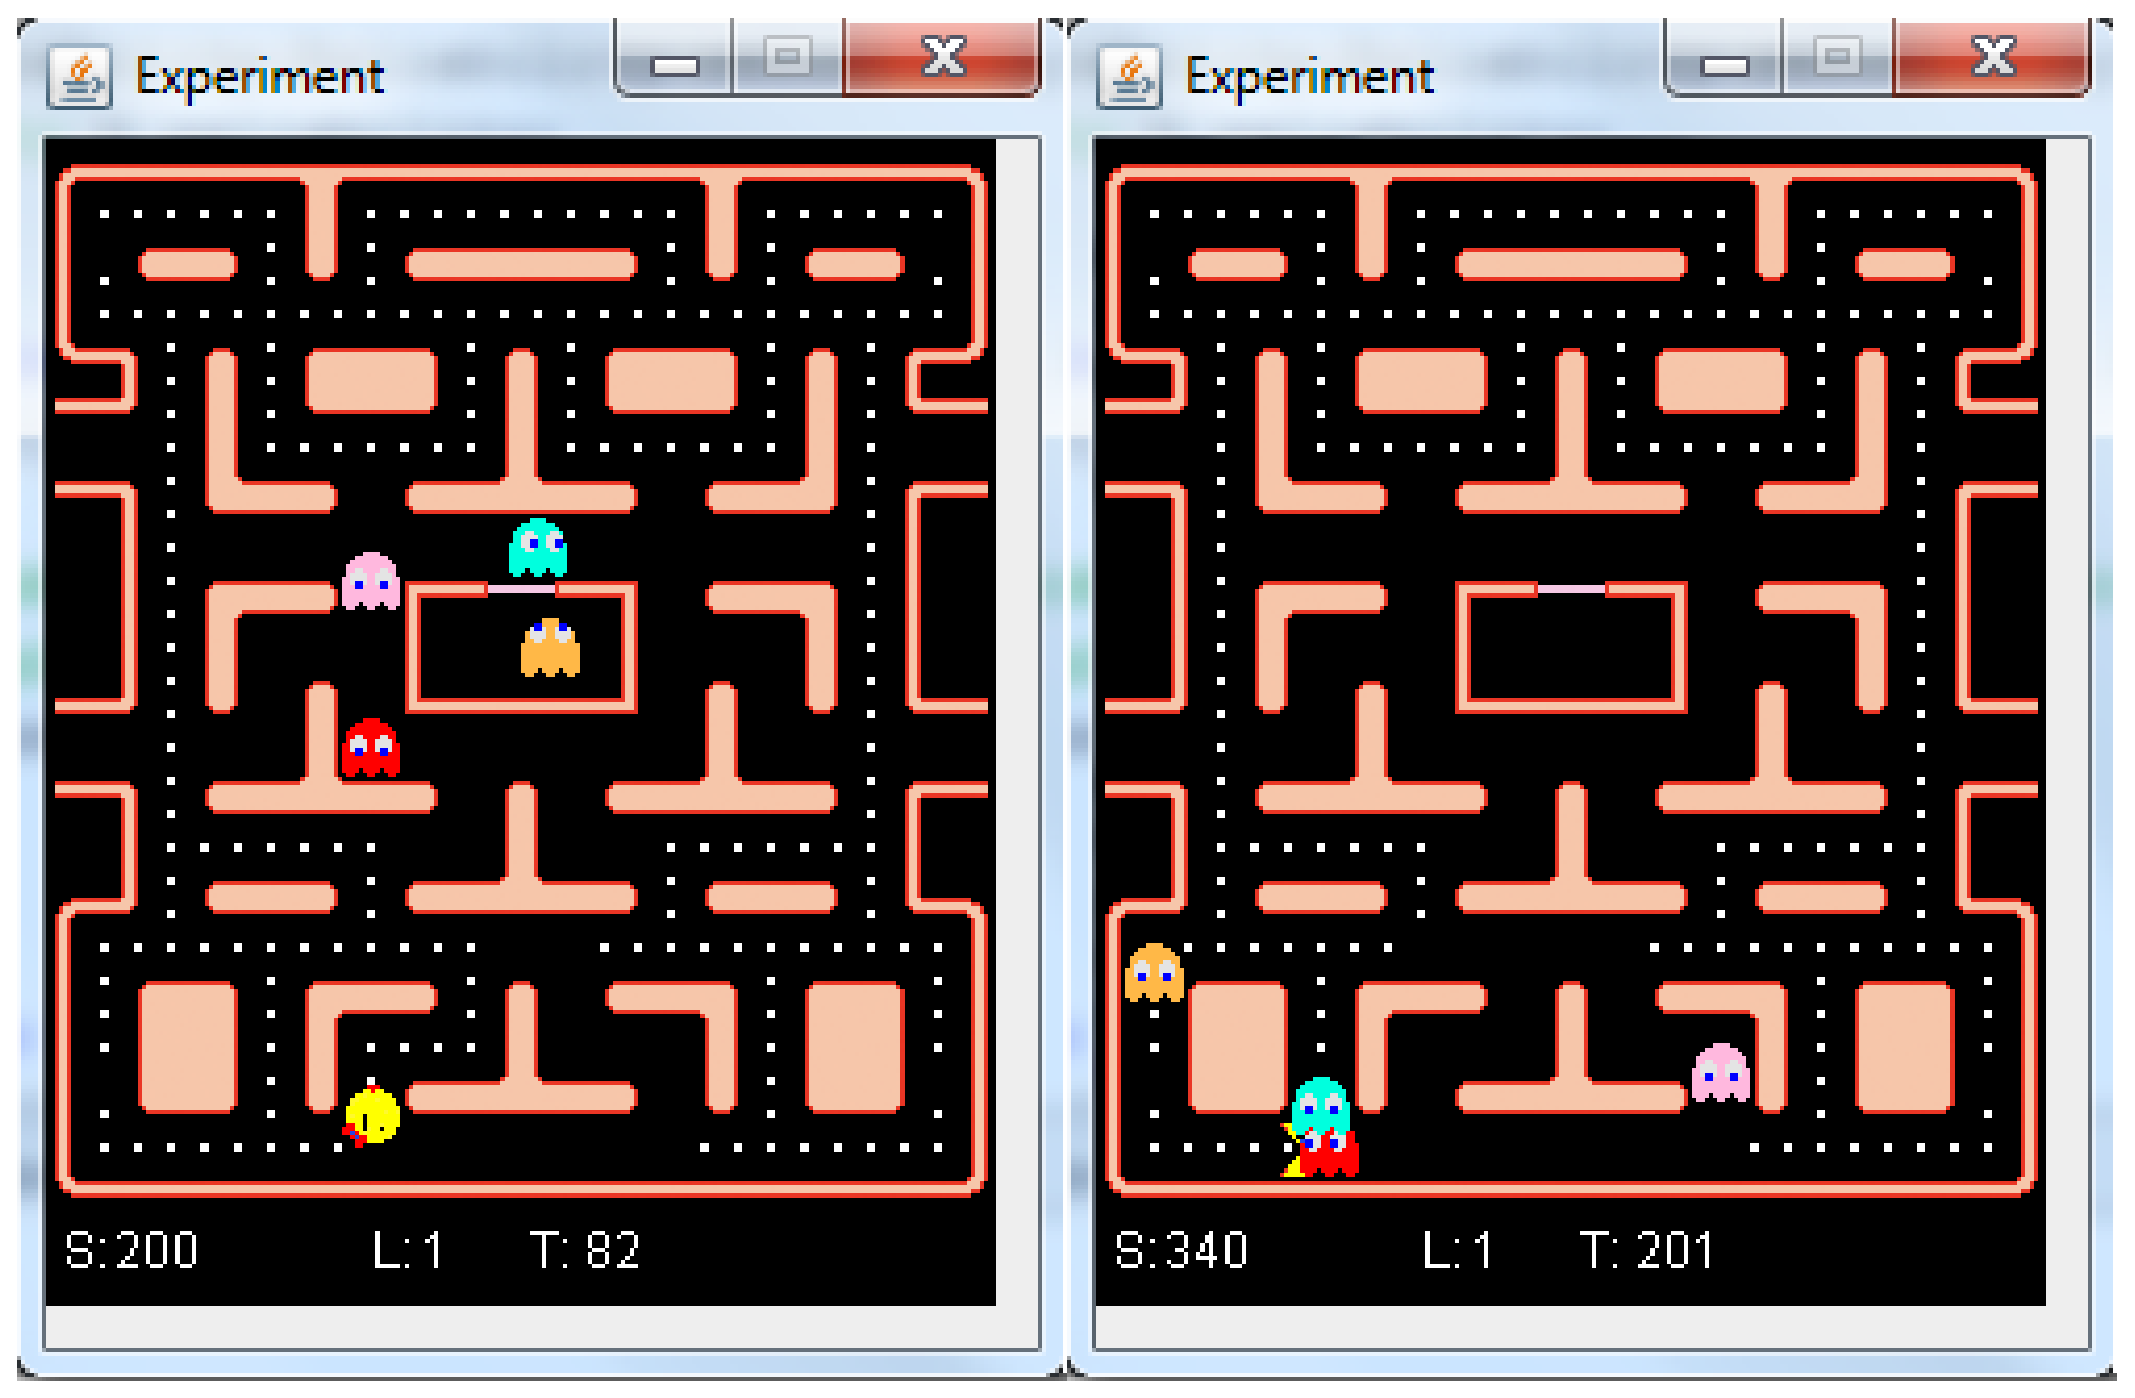
\includegraphics[width=14cm]{img/pacman_framework.eps}
\end{center}
\caption{\footnotesize Game of Ms Pacman.}{\footnotesize Left picture shows the game few moments after it began. Three
ghosts started to hunt the Pac-Man while the orange one is still waiting in lair. Right
picture, on the other hand, shows the game just before the end. Pac-Man does not have any
escape path and is being caught with in a while with no life remaining.}
\label{fig_pacman_framework}
\end{figure}

Pac-Man has the same movement speed as non-edible ghosts. Paths inside the maze are divided
into small segments, four between two neighbouring pills. Pac-Man has to play an action after
at each segment, turning back in the middle of path or at the crossroad is allowed and so
Pac-Man has always at least two action to choose between. Contrarily, ghosts' movement is
restricted. Additional rule on ghosts' movement is that ghosts cannot turn back in the middle
of a path nor at a crossroad. That means that once a ghost chooses one way from a crossroad, it
has to continue to the end of the path. Despite of that, ghosts have to play an action on each
segment even though there is only one action to choose from.

\todo{Porovnat Pac-Mana s pursuit-evation game}

So Pac-Man and ghosts play their actions at each segment of the maze but they, of course, have
to play an action in a limited time. Ms Pac-Man vs Ghosts framework provides by default 40 ms
to play what corresponds with the natural game timing when a human player controls Pac-Man.

\subsection{Framework details}

In our thesis, we use Ms Ghost vs Pacman framework version 6.2. The framework is written in
Java what simplifies the development of controllers of the players. In original game, player
was able to control only Pac-Man and ghosts were controlled by simple AI. In the framework,
it is also possible to develop controller for the ghosts. The only work a user is supposed to 
do is
implement a controller of Pac-Man or ghosts, methods for running a game or a set of games are
prepared for usage. 

A player controller is a class implementing an interface having only one
method. In case of ghosts controller, method's header is \texttt{public EnumMap<GHOST,MOVE>
getMove(Game game,long timeDue)}, where \texttt{EnumMap<GHOST,MOVE>} is a joint-action of
ghosts, \texttt{game} contains information of current game and \texttt{timeDue} contains time
until which the method has to return an action.
If an action is not returned on time, certain
default action is chosen by framework itself.

\todo{Tady je možné ještě popsat, že jsem si upravil i metody na běh experimentů}

\subsection{Pac-Man Opponent}

To evaluate the strength of ghost controllers based on distributed MCTS algorithms, we need to
choose appropriate Pac-Man opponent to play against. Unfortunately, experiments with Pac-Man
controllers included in Ms Pacman vs Ghosts framework showed that these controllers are too
weak for evaluation. Thus, it was necessary to look for better Pac-Man controllers. 

Main purpose of the Ms Pacman vs Ghosts project is organizing competitions between existing
controllers. Competitions are usually held on various conferences and meanwhile there is also a
league  in which all controllers commited into the website compete. Thanks to the leagure
results we were able to contact authors of the league leading Pac-Man and obtained source code
of ICEP\_IDDFS \ref{IcepIddfs} what is controller based on iterative deepening depth-first
search approach. We haven't received more details about the controller. However, experiments
running against it give promising results and so the controller was chosen as an opponent to
compare with.


\section{Implementation Notes}

In this section, we will discuss important implementation details of our controllers. As
mentioned in previous section, framework used for the experiments is written in Java and so
controllers are also supposed to be written in this language.


\subsection{Tree construction}

Here we will talk about the way the concrete realization of MCTS tree for the game of Ms
Pac-Man. The most direct approach to a construction is to keep a node of the tree for each game
step and store, besides the value and the visit count, actions performed by Pac-Man and all
ghosts. By exposing and resolving of problems of this solution, we have reached the
construction used in our controllers.

First problem to be solved is that MCTS tree should not work with simultaneous plays of
multiple teams as discussed in \ref{sec_two_players_mcts}. Section 
\ref{sec_turn_based_game_conversion} gives us a recipe to deal with simultaneous moves by
convertion of a simultaneous game to a turn-based game by splitting simultaneous nodes. The
conversion is not done on the unterlying Ms Pac-Man game itself but only for purposes of
expansion of nodes. When a simultaneous node is being expanded, instead of creating of a child
node for each pacman-ghosts joint-action, only children for each pacman action is created and
each of this children is immediately expanded with ghosts actions. By this approach,
simultaneous nodes are splitted accordingly to optimistic expansion since in such a tree the
ghosts suppose to know the action of Pac-Man played in the simultaneous node. Our
implementation, in addition, supports the pesimistic expansion where ghosts actions are
expanded first in simultaneous nodes.

Second problem is quite high branching factor caused by Pac-Man which is able to change its
direction any time. To reduce the branching factor, we consider additional rules of Pac-Man's
movement for purposes of node expansion. We allow Pac-Man to change its direction only at
crossroads, in the neighbourhood of a segment with not yet eaten power pill and at segments in
the middle of path when last segment allowing the direction change is exactly 6 segments far.
When computing the MCTS tree for Pac-Man, this reduction does not bring any difficulty since
the player controlled by the algorithm follows additional rules. But when Pac-Man is an
opponent of the algorithm, it may play an action not corresponding with these rules what
directly leads to desynchronization between game state and built tree. Next time any ghost
reaches  a crossroad and the desynchronization is detected, ghost play an action accordingly to
the tree but then instead of using a subtree defined by the action for further computations,
new tree is built from scratch.

Finally, after expansion of simultaneous nodes and reduction of Pac-Man moves, the tree
will contain nodes having only one child which are also removed what adds a necessity to keep
lengths of edges between nodes.


\subsection{Communication}

Main method of a player controller (\texttt{getMove}) returns the joint-action
(\texttt{EnumMap<GHOST,MOVE>}) of the ghosts
but for purposes of distributed approach, each ghost is supposed to reason individually 
returning its action. To fulfil this, four subcontrollers, returning single \texttt{MOVE}
actions are started in four separated threads and virtual bidirectional communication 
channels are created between each pair of subcontrollers.

Channels provide interfaces for both senders and receivers and work with real time. Channel
consists of queue of messages to be sent and queue of received messages. Messages from the
sending queue to the receiving queue are transmitted every time a method on a channel is
called. Amount of messages transmitted corresponds with time elapsed since last channel event
ending with nonempty sending queue.

For purposes of evaluation of robustness of distributed algorithms againts communication
failures, channels contain a reliability object which simulates a reliability of a channel.
After a transmission of each message, the object determine if the message is really transmitted
to the receiver or if a failure occured and the message has to be discarded. Exact way of
reasoning of the reliability object is described in Section \ref{sec_methodics}.


\section{Methodics}
\label{sec_methodics}

\section{MCTS Tuning}

\section{Comparison of the Algorithms}

\section{Conclusion}
